\graphicspath{{"Appendix/figures/Smoothmax"}}

\chapter{Smoothmax Function}
\label{chap:smoothmax-proof}

\shortAbstract{
    Boolean operations such as union, intersection, and difference are fundamental in logic and have been widely adopted in computer graphics, particularly in Constructive Solid Geometry (CSG). In this context, they are used to combine geometric primitives into complex shapes. However, while Boolean functions are naturally discontinuous, modern rendering pipelines typically favor smoothness to enable effects like anti-aliasing, gradient shading, and physical simulation. This has led to the development of smooth operators: continuous, differentiable approximations of Boolean functions. The ideal objective is to construct operators that are not only smooth but infinitely differentiable, also known as functions belonging to the class $C^\infty$.
}

\section{Definition of the Smoothmax function $\smoothmax$}

In \cref{subsubsec:height-functions-blending}, we introduced the operator $\smoothmax: \R^2 \to \R$ as a smooth approximation of the $\max$ operator, defined with the sharpness parameter $k > 0$ as:

\begin{align}
    \smoothmax(a, b) = a + \frac{1}{2} \cdot \frac{b - a}{1 + e^{-k(b - a)}} + \frac{1}{2} \cdot \frac{b - a}{1 - e^{-k(b - a)}}
\end{align}

We observe that for $a = b$, the final term becomes undefined due to a removable singularity in the expression $\frac{b - a}{1 - e^{-k(b - a)}}$, potentially introducing a discontinuity. In this section, we demonstrate that this function is in fact continuous on $\R^2$ and is infinitely differentiable, i.e., $\smoothmax \in C^\infty$.

It is evident that the only potentially problematic term in $\smoothmax$ is $\frac{b - a}{1 - e^{-k(b - a)}}$, as the rest of the expression is composed of standard smooth ($C^\infty$) functions.

To simplify our analysis, define the auxiliary function:

\begin{align}
    f(x) = \frac{x}{1 - e^{-kx}}
\end{align}

Then we may express:

\begin{align}
    \smoothmax(a, b) = a + \frac{1}{2} \cdot \frac{b - a}{1 + e^{-k(b - a)}} + \frac{1}{2} f(b - a)
\end{align}

To assess the continuity and differentiability of $\smoothmax$, it suffices to analyze $f$ in a neighborhood of $x = 0$, where the apparent singularity arises.

\begin{figure}
    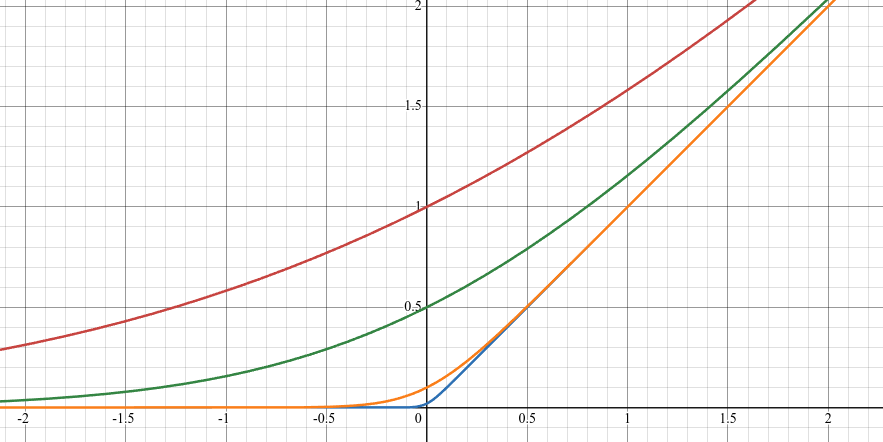
\includegraphics[width=\linewidth]{Smoothmax_f_graph.png}
    \caption{Plotting the function $f(x)$ suggests continuity, with the sharpness parameter $k$ equal to 1, 2, 5, 10 for the curves red, green, orange and blue respectively; although it is initially undefined at $x = 0$.}
    \label{fig:smoothmax-f-plot}
\end{figure}

\section{Continuity: $C^0$}

From \cref{fig:smoothmax-f-plot}, we observe that $f$ appears continuous at $x = 0$. However, directly evaluating $f(0)$ yields the indeterminate form $\frac{0}{0}$. To resolve this, we apply L'Hôpital's Rule:

\begin{align}
    \lim_{x \to 0} f(x) = \lim_{x \to 0} \frac{x}{1 - e^{-kx}} = \frac{g'(x)}{h'(x)}
\end{align}
where
\begin{align}
    g(x) = x, \quad & \quad g'(x) = 1 \\
    h(x) = 1 - e^{-kx}, \quad & \quad h'(x) = k e^{-kx}
\end{align}

Thus,
\begin{align}
    \lim_{x \to 0} \frac{g'(x)}{h'(x)} = \lim_{x \to 0} \frac{1}{k e^{-kx}} = \frac{1}{k}
\end{align}

Since the limit exists and equals $\frac{1}{k}$, we define:

\begin{align}
    f(0) := \frac{1}{k}
\end{align}

This definition removes the singularity and ensures that $f$ is continuous on $\R$. For the case $a = b$, we then have:

\begin{align}
    \smoothmax(a, b) = a + \frac{1}{2k}
\end{align}

The complete definitions of the functions are:

\begin{align}
    f(x) &= \begin{dcases}
        \frac{x}{1 - e^{-kx}} &, x \neq 0 \\
        \frac{1}{k} &, x = 0
    \end{dcases} \\
    \smoothmax(a, b) &= \begin{dcases}
        a + \frac{1}{2} \cdot \frac{b - a}{1 + e^{-k(b - a)}} + \frac{1}{2} \cdot \frac{b - a}{1 - e^{-k(b - a)}} &, a \neq b \\
        a + \frac{1}{2k} &, a = b
    \end{dcases}
\end{align}

We have shown that $f$ is continuous on $\R$, and thus $\smoothmax$ is continuous on $\R^2$, meaning $\smoothmax \in C^0$.
\section{Smoothness: $C^\infty$}

In this section, we prove that $\smoothmax$ is infinitely differentiable. Since it is composed of standard smooth functions and the auxiliary function $f(x) = \frac{x}{1 - e^{-kx}}$, it suffices to show that $f \in C^\infty(\R)$.

We prove this by induction on the number of derivatives of $f$.

\begin{Itemize}
    \Item{$\bullet$} \textbf{Base case:} As shown earlier, $f$ is continuous on $\R$ with the singularity at $x = 0$ removed by defining $f(0) := \frac{1}{k}$. Hence, $f \in C^0$.

    \Item{$\bullet$} \textbf{Inductive step:} Assume that $f^{(n)}$ exists, is continuous on $\R$, and is expressible in the form
    \begin{align}
        f^{(n)}(x) = \frac{P_n(x, e^{-kx})}{(1 - e^{-kx})^{n+1}},
    \end{align}
    where $P_n$ is a smooth function of $x$ and $e^{-kx}$. This form arises naturally from repeated applications of the quotient and chain rules:
    
    \begin{itemize}
        \item The denominator gains a factor of $(1 - e^{-kx})$ with each differentiation, hence the power $(n+1)$.
        \item The numerator $P_n$ is a recursively constructed smooth function resulting from differentiation of $P_{n-1}$ and the chain rule applied to $e^{-kx}$. Since $e^{-kx}$ is smooth and all operations preserve smoothness, $P_n(x, e^{-kx})$ remains smooth.
    \end{itemize}
    
    Differentiating $f^{(n)}$ using the quotient rule $\left(\frac{u}{v}\right)' = \frac{u' v - u v'}{v^2}$, we get:
    \begin{align}
        f^{(n+1)}(x) = \frac{d}{dx} \left( \frac{P_n(x, e^{-kx})}{(1 - e^{-kx})^{n+1}} \right)
    \end{align}
    which results in a new expression:
    \begin{align}
        f^{(n+1)}(x) = \frac{P_{n+1}(x, e^{-kx})}{(1 - e^{-kx})^{n+2}},
    \end{align}
    where $P_{n+1}$ is again a smooth function of $x$ and $e^{-kx}$, obtained via product, chain, and sum rules. Importantly, we do not need the explicit form of $P_{n+1}$, it suffices to know it is smooth.

    At $x = 0$, both numerator and denominator vanish, but to the same order: the denominator vanishes to order $n+2$ due to the Taylor expansion
    \begin{align}
        1 - e^{-kx} = kx - \frac{k^2 x^2}{2} + \frac{k^3 x^3}{6} - \frac{k^4 x^4}{24} + \frac{k^5 x^5}{120} + O(x^6)
    \end{align}
    and $P_{n+1}(x, e^{-kx})$ also vanishes to order at least $n+2$ due to the construction. Thus, any singularity at $x = 0$ is removable, and $f^{(n+1)}$ can be continuously extended there.
\end{Itemize}

By induction, $f^{(n)}$ exists and is continuous for all $n \geq 0$, so $f \in C^\infty(\R)$. Since $\smoothmax$ is built from smooth functions and $f$, we conclude that $\smoothmax \in C^\infty(\R^2)$.

\smallConclusion

Moreover, since $f(x) = \frac{x}{1 - e^{-kx}}$ is composed of analytic functions with a removable singularity at $x = 0$, $f$ is real-analytic on $\R$. Consequently, $\smoothmax$ is also real-analytic on $\R^2$.

\section{Practical expressions for $\smoothmax(a, b)$ and its derivatives}
\label{sec:smoothmax-practical-forms}

In applications such as shading, soft blending, and physical simulation, efficient evaluation of $\smoothmax(a, b)$ and its first and second derivatives is often required. This section provides compact, implementation-ready expressions for these quantities.

\subsection*{Function value}
\begin{align}
    \smoothmax(a, b) &= \begin{cases}
        a + \frac{(b - a)}{2} \left( \frac{1}{1 + e^{-k(b-a)}} + \frac{1}{1 - e^{-k(b-a)}} \right) &\text{if } a \neq b \\
        a + \frac{1}{2k} &\text{if } a = b
    \end{cases}
\end{align}

\subsection*{First derivatives}
\begin{align}
    \frac{\partial}{\partial a} \smoothmax(a, b) &= - g_1(a, b) \\
    \frac{\partial}{\partial b} \smoothmax(a, b) &= g_1(a, b)
\end{align}

with 
\begin{align}
    g_1(a, b) = \begin{cases}
        \frac{e^{2k(b-a)}\left(e^{2k(b-a)} - 1\right)}{\left(e^{2k(b-a)}-1\right)^2} &\text{if } a \neq b \\
        \frac{1}{2} &\text{if } a = b
    \end{cases}
\end{align}

\subsection*{Second derivatives}
\begin{align}
    \frac{\partial^2}{\partial a^2} \smoothmax(a, b) = \frac{\partial^2}{\partial b^2} \smoothmax(a, b) = - g_2(a, b) \\
    \frac{\partial^2}{\partial a \partial b} \smoothmax(a, b) = \frac{\partial^2}{\partial b \partial a} \smoothmax(a, b) = g_2(a, b)
\end{align}

where the second derivative of the core function is given by:
\begin{align}
    g_2(a, b) = \begin{cases}
        \frac{4ke^{2ka}e^{2kb} \left( e^{2ka} (ka-kb-1) + e^{2kb}(ka - kb + 1) \right)}{\left(e^{2kb}-e^{2ka} \right)^3} &\text{if } a \neq b \\
        0  &\text{if } a = b
    \end{cases}
\end{align}

The expression is algebraically heavy, but all terms are composed of simple exponentials, products, and powers, making it fast and safe to compute in practice, and the redundant components an be cached. At $x = 0$, we have $g_2(0) = 0$ by symmetry and smoothness of the underlying expression.

A $\smoothmin$ operator can be derived directly from the $\smoothmax$ by reversing the sign of the sharpness parameter $k_{\text{smoothmin}} = - k_{\text{smoothmax}}$.



\section{Comparison with other smooth maximum functions}
\label{sec:comparison-smoothmax}

To evaluate the practical performance of our \texttt{smoothmax} operator, we compared it with two commonly used alternatives:

\begin{itemize}
    \item \textbf{LogSumExp:}
    \begin{align}
        \mathrm{LSE}(a, b) = \frac{1}{k} \log\left(e^{k a} + e^{k b}\right)
    \end{align}
    This is a popular smooth approximation to $\max(a, b)$, widely used in machine learning.

    \item \textbf{Smooth Absolute Max:}
    \begin{align}
        \mathrm{AbsMax}(a, b) = \frac{a + b}{2} + \frac{1}{2k} \log\left(1 + e^{-k|a - b|}\right)
    \end{align}
    A symmetric blend of the average and the absolute difference.

    \item \textbf{Smoothmax (ours):}
    \begin{align}
        \smoothmax(a, b) = a + \frac{b - a}{2} \left( \frac{1}{1 + e^{-k(b - a)}} + \frac{1}{1 - e^{-k(b - a)}} \right)
    \end{align}
    Our symmetric and infinitely differentiable approximation, designed to behave well under chaining and small sharpness variations.
\end{itemize}

We compare these functions across four benchmarks: chaining behavior, sharpness resolution, runtime performance, and aggregation error.

\subsection*{Chaining behavior}

We evaluate each operator by chaining it over $n$ inputs drawn randomly from $[0, 100]$. The true maximum is compared to the approximate maximum, and errors are averaged over 100 trials per $n$.

\begin{figure}[H]
    \centering
    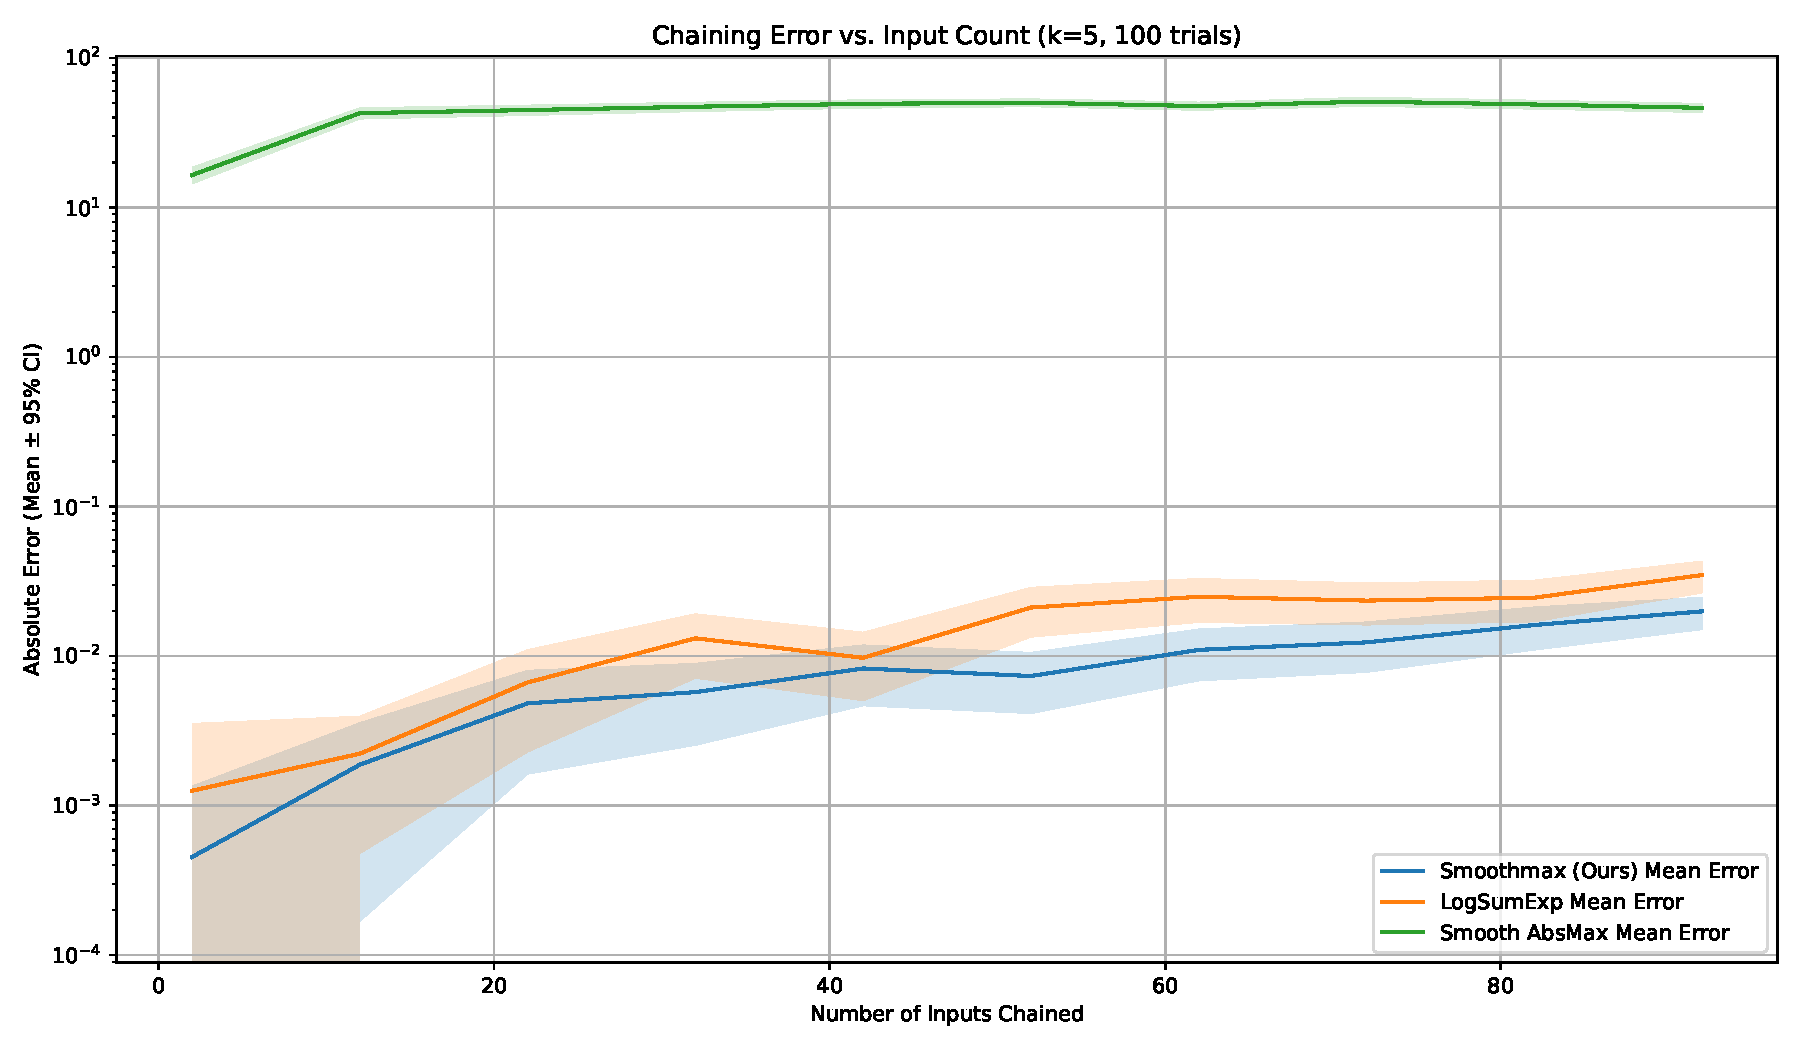
\includegraphics[width=0.8\linewidth]{compare_chaining.pdf}
    \caption{Mean absolute error as more values are chained together ($k = 5$).}
\end{figure}

\begin{table}[H]
\centering
\begin{tabular}{l|ccc}
    \toprule
    Function & Mean error & Std dev & 95th percentile \\
    \midrule
    Smoothmax & $7.91 \times 10^{-3}$ & $1.93 \times 10^{-2}$ & $6.02 \times 10^{-2}$ \\
    LogSumExp & $1.15 \times 10^{-2}$ & $2.62 \times 10^{-2}$ & $6.30 \times 10^{-2}$ \\
    AbsMax    & $5.01 \times 10^{1}$  & $1.81 \times 10^{1}$  & $7.77 \times 10^{1}$ \\
    \bottomrule
\end{tabular}
\caption{Error statistics over the aggregation of 50 random values in [0, 100] ($k = 5$)}
\end{table}

\subsection*{Precision and sharpness}

We also test how each function converges to $\max(a, b)$ as sharpness $k$ increases. We fix two very close inputs $a = 1.0000$ and $b = 1.0001$ and sweep $k$ over several orders of magnitude. We see in \cref{fig:smoothmax-sharpness} that for small values of $k$, the AbsMax operator is closer to the ground truth, but as $k$ tends to exaggerated high values, our smoothmax operator gets significantly more accurate.

\begin{figure}[H]
    \centering
    \autofitgraphics[width=0.8\linewidth]{compare_sharpness-low-values.pdf, compare_sharpness.pdf}
    \caption{Approximation error as a function of $k$.}
    \label{fig:smoothmax-sharpness}
\end{figure}

\subsection*{Runtime benchmark}

To get a rough idea of performance, we measured the average time (in microseconds) for a single call of each function over 10000 repetitions, using scalar inputs and $k = 5$. This test was conducted with using Python 3.10 and NumPy 1.25 on a Linux system with a modern multi-core CPU and 14GB of RAM. 

\begin{table}[H]
\centering
\begin{tabular}{l|c}
    \toprule
    Function & Time \\
    \midrule
    Smoothmax & 1.40 \\
    LogSumExp & 2.68 \\
    AbsMax    & 1.80 \\
    \bottomrule
\end{tabular}
\caption{Average runtime per call (in $\mu$s)}
\end{table}

\midConclusion

Overall, \texttt{smoothmax} performs best across the board:
\begin{itemize}
    \item It keeps errors low even when chaining over many values.
    \item It converges smoothly and accurately as sharpness increases.
    \item It is fast to compute and numerically stable.
\end{itemize}

This makes it a practical and robust replacement for $\max(a, b)$ in graphics and simulation tasks where smoothness matters.